\documentclass[11pt,a4paper]{article}

\usepackage[utf8]{inputenc}
\usepackage[T1]{fontenc}
\usepackage{geometry}
\usepackage{graphicx}
\usepackage{booktabs}
\usepackage{longtable}
\usepackage{array}
\usepackage{float}
\usepackage{hyperref}
\usepackage{xcolor}
\usepackage{listings}
\usepackage{caption}

\geometry{margin=1in}
\setlength{\emergencystretch}{3em}
\hypersetup{
  colorlinks=true,
  linkcolor=blue,
  urlcolor=blue,
  citecolor=blue
}

\definecolor{codebg}{RGB}{248,248,248}
\definecolor{codecomment}{RGB}{0,110,0}
\definecolor{codekeyword}{RGB}{0,0,150}

\lstdefinestyle{pythonstyle}{
  language=Python,
  basicstyle=\ttfamily\footnotesize,
  backgroundcolor=\color{codebg},
  keywordstyle=\color{codekeyword}\bfseries,
  commentstyle=\color{codecomment},
  showstringspaces=false,
  breaklines=true,
  frame=single,
  tabsize=4
}

\title{Phase II Project Report\\RetailHero Uplift Modeling: CCP vs CCU Evaluation}
\author{Aniket}
\date{29 April 2026}

\begin{document}

\maketitle

\begin{abstract}
This report documents the Phase II implementation of a value-aware uplift-modeling pipeline for the RetailHero / X5 retail intervention dataset. The work extends Phase I, which established that the campaign was effectively randomized, that the average treatment effect was modest, and that response heterogeneity was large enough to justify uplift modeling. Phase II operationalizes that finding by comparing a standard customer purchase-propensity baseline (CCP) against three customer churn uplift (CCU) estimators under one reproducible evaluation framework. The pipeline rebuilds features directly from the raw CSV files, trains all models on the full extracted dataset, evaluates them on a stratified holdout set, and reports Qini, liftup, predictive maximum profit, and maximum profit uplift. The final result is that the uplift random forest is the strongest incremental-targeting model, outperforming the CCP baseline on uplift-specific metrics while preserving a transparent, reproducible workflow.
\end{abstract}

\tableofcontents
\newpage

\section{Project Objective}
The objective of Phase II was to implement a defensible, reproducible comparison between:
\begin{itemize}
    \item \textbf{Model A: CCP baseline}, a standard purchase-propensity model trained only on the control group.
    \item \textbf{Model B: CCU models}, uplift estimators that rank customers by expected incremental response to treatment.
\end{itemize}

The practical research question is:
\begin{quote}
Can the intervention be targeted more efficiently by ranking customers on expected incremental value rather than raw purchase likelihood?
\end{quote}

This framing matters because a customer who is highly likely to buy anyway may still be a poor target for campaign spend. Uplift modeling is valuable only if it changes that ranking in a measurable and profitable way.

\section{Data and Verified Phase I Findings}
\subsection{Dataset}
The project uses the RetailHero uplift dataset with the following raw inputs:
\begin{itemize}
    \item \texttt{clients.csv}
    \item \texttt{products.csv}
    \item \texttt{purchases.csv}
    \item \texttt{uplift\_train.csv}
    \item \texttt{uplift\_test.csv}
    \item \texttt{uplift\_sample\_submission.csv}
\end{itemize}

The purchases file is the dominant data asset and contains approximately 4.4 GB of transaction history. Because of its size, the implementation uses DuckDB-backed SQL aggregation rather than loading the entire file into a single in-memory pandas frame.

\subsection{Phase I Findings Revalidated from Raw Data}
Phase I findings were rechecked directly from raw data via the verification script rather than relying on notebook narrative alone. The key findings are summarized in Table~\ref{tab:phase1}.

\begin{table}[H]
\centering
\caption{Verified Phase I findings used to motivate Phase II}
\label{tab:phase1}
\begin{tabular}{p{0.46\textwidth} p{0.42\textwidth}}
\toprule
\textbf{Finding} & \textbf{Verified value} \\
\midrule
Treatment / control ratio & 0.999230 (99{,}981 treated / 100{,}058 control) \\
Baseline uplift & 3.323 percentage points \\
Average uplift in low-frequency deciles 0--3 & 4.452 percentage points \\
Average uplift in high-frequency deciles 6--9 & 1.755 percentage points \\
Sure Things share & 30.176\% of training clients \\
Age anomalies & min = -7{,}491, max = 1{,}901, flagged = 1{,}145 \\
Distinct non-null \texttt{level\_1} categories & 3 \\
Test-set clients with purchase history & 200{,}123 / 200{,}123 \\
\bottomrule
\end{tabular}
\end{table}

\subsection{Why These Findings Justify Phase II}
These findings defend the Phase II design in three ways:
\begin{enumerate}
    \item The near-perfect treatment/control balance means uplift estimates can be interpreted causally without heavy post-hoc adjustment.
    \item The modest average treatment effect means a single global response model is likely to be wasteful because the mean hides heterogeneity.
    \item The concentration of uplift among lower-frequency customers means targeting by purchase probability alone is not aligned with incremental value.
\end{enumerate}

\section{Phase II Methodology}
\subsection{Design Principles}
Phase II was built around four design principles:
\begin{enumerate}
    \item \textbf{Raw-data-first reproducibility}: all Phase II features are rebuilt from \texttt{data/*.csv} rather than notebook-only exports.
    \item \textbf{Comparable feature space}: all models consume the same deterministic numeric feature matrix.
    \item \textbf{Value-aware evaluation}: uplift models are not judged only by response prediction, but by incremental targeting value.
    \item \textbf{Transparent implementation}: the pipeline is organized into feature, model, metric, and orchestration modules rather than one monolithic script.
\end{enumerate}

\subsection{Feature Engineering}
The final Phase II matrix contains 44 numeric features with zero missing values after deterministic filling and explicit missingness indicators. The feature groups are:
\begin{itemize}
    \item \textbf{Demographics}: \texttt{age}, \texttt{age\_clean}, \texttt{age\_flagged}, gender indicators, \texttt{gender\_known}
    \item \textbf{Redemption behavior}: redeemed flag, time-to-redeem, card tenure, and redemption recency
    \item \textbf{Purchase behavior}: spend, transactions, trips, items, basket metrics, stores, products, points, recency, tenure
    \item \textbf{Product behavior}: alcohol spend share, own-trademark spend share, netto aggregates, spend-share across the three \texttt{level\_1} groups, and brand concentration (HHI)
\end{itemize}

This design is defensible because it follows directly from Phase I. The hashed category hierarchy is not semantically interpretable, so the implementation does not pretend it is. Instead, it transforms product metadata into client-level behavioral features that can still carry signal.

\subsection{Data Split}
The Phase II pipeline uses:
\begin{itemize}
    \item an outer holdout split of 20\% of \texttt{uplift\_train} for validation,
    \item stratification on the joint label \texttt{(treatment\_flg, target)},
    \item a fixed random seed of 123,
    \item a smaller inner tuning split inside the training fold only.
\end{itemize}

This is the correct compromise for the current stage of the project. It preserves a clean validation set while keeping the implementation simple enough to inspect and rerun.

\subsection{Models}
\subsubsection{Model A: CCP baseline}
The CCP baseline is an \texttt{XGBClassifier} trained on control-group rows only. It predicts purchase propensity rather than treatment effect.

This design is defensible because:
\begin{itemize}
    \item it creates a strong conventional benchmark,
    \item it avoids learning treatment-induced behavior when estimating organic purchase likelihood,
    \item it is exactly the sort of model a business team might deploy if uplift were ignored.
\end{itemize}

\subsubsection{Model B1: Two-model logistic uplift}
Two separate regularized logistic models are trained, one on treated customers and one on control customers. The uplift score is:
\[
\hat{u}(x) = \hat{P}(Y=1 \mid T=1, X=x) - \hat{P}(Y=1 \mid T=0, X=x)
\]

This is the most literal implementation of the roadmap formula.

\subsubsection{Model B2: Lo-style interaction logistic uplift}
A single logistic model is trained on all rows with:
\begin{itemize}
    \item the treatment indicator as a feature,
    \item first-order interactions between treatment and all covariates.
\end{itemize}
The uplift score is obtained by scoring each customer twice, once under treatment and once under control, then taking the difference.

This is defensible because it provides a structured single-model alternative to the two-model approach.

\subsubsection{Model B3: Uplift random forest}
The non-linear uplift model is implemented using \texttt{causalml}'s \texttt{UpliftRandomForestClassifier} with:
\begin{itemize}
    \item \texttt{KL} split evaluation,
    \item string-encoded treatment labels required by the package API,
    \item light tuning over tree count, feature count, depth, leaf size, and regularization.
\end{itemize}

This is defensible because it is the most expressive model in the comparison and can capture non-linear treatment heterogeneity that linear models cannot.

\subsection{Evaluation Framework}
Phase II evaluates the models with four complementary views:
\begin{itemize}
    \item \textbf{Qini curves}: how well the model ranks incremental responders
    \item \textbf{Liftup curves}: uplift-specific analogues of lift behavior
    \item \textbf{Predictive maximum profit (MP)}: used for the CCP benchmark
    \item \textbf{Maximum profit uplift (MPU)}: used for incremental targeting
\end{itemize}

The default economics are:
\begin{itemize}
    \item average basket value = empirical average trip value = 4425.003 RUB
    \item SMS cost = 1 RUB
\end{itemize}

Sensitivity analysis then varies both assumptions.

\section{Implementation Summary}
\subsection{Code Organization}
The Phase II codebase is modular:
\begin{itemize}
    \item \texttt{phase2\_features.py}: raw-data feature construction and cache writing
    \item \texttt{phase2\_models.py}: model wrappers, tuning, and scoring
    \item \texttt{phase2\_metrics.py}: ranking, Qini, liftup, MP, and MPU calculations
    \item \texttt{phase2\_pipeline.py}: full orchestration and artifact generation
    \item \texttt{verify\_phase2\_outputs.py}: artifact and consistency checks
\end{itemize}

\subsection{Implementation Integrity Checks}
The completed pipeline passed all current verification checks:
\begin{itemize}
    \item 200{,}039 Phase II train rows and 200{,}123 Phase II test rows
    \item 44 model features
    \item zero missing feature values in both train and test matrices
    \item valid category-share algebra with maximum absolute error $1.343 \times 10^{-14}$
    \item finite validation and test scores for all four models
    \item valid target-share bounds for Qini, liftup, and sensitivity outputs
\end{itemize}

This matters because a submission-ready report should not only present model outcomes; it should demonstrate that the pipeline itself is internally coherent.

\section{Results}
\subsection{Selected Hyperparameters}
The final selected hyperparameters from the current full run are shown in Table~\ref{tab:params}.

\begin{table}[H]
\centering
\caption{Selected model hyperparameters}
\label{tab:params}
\begin{tabular}{p{0.26\textwidth} p{0.62\textwidth}}
\toprule
\textbf{Model} & \textbf{Selected parameters} \\
\midrule
Model A - CCP baseline & \texttt{n\_estimators=250}, \texttt{max\_depth=3}, \texttt{learning\_rate=0.05}, \texttt{subsample=0.85}, \texttt{colsample\_bytree=0.85} \\
Model B1 - Two-model logistic & \texttt{C=1.0} \\
Model B2 - Lo interaction logistic & \texttt{C=10.0} \\
Model B3 - Uplift random forest & \texttt{n\_estimators=25}, \texttt{max\_features=12}, \texttt{max\_depth=5}, \texttt{min\_samples\_leaf=100}, \texttt{min\_samples\_treatment=50}, \texttt{n\_reg=10} \\
\bottomrule
\end{tabular}
\end{table}

\subsection{Validation Summary}
The full validation summary is shown in Table~\ref{tab:results}. The validation holdout contains 40{,}008 rows.

\begin{table}[H]
\centering
\caption{Phase II validation summary}
\label{tab:results}
\small
\resizebox{\textwidth}{!}{
\begin{tabular}{p{0.29\textwidth} r r r r}
\toprule
\textbf{Model} & \textbf{Qini AUC} & \textbf{Top-decile liftup} & \textbf{MPU} & \textbf{Optimal target share} \\
\midrule
Model B3 - CCU Uplift Random Forest & 0.004759 & 3.637315 & 158.307694 & 0.7475 \\
Model B1 - CCU Two-Model Logistic & 0.003297 & 3.239985 & 146.083912 & 1.0000 \\
Model B2 - CCU Lo Interaction Logistic & 0.003245 & 3.231146 & 146.083912 & 1.0000 \\
Model A - CCP Baseline & -0.002239 & 0.016284 & 146.083912 & 1.0000 \\
\bottomrule
\end{tabular}
}
\normalsize
\end{table}

For completeness, the CCP baseline also achieved a predictive maximum profit of 2742.063982 under the default economics. That figure is intentionally reported separately from MPU because it is not the same business question. Predictive MP rewards finding likely buyers. MPU rewards finding customers whose behavior is changed by treatment. Those are related but not interchangeable objectives.

\subsection{Interpretation}
Three findings matter most:
\begin{enumerate}
    \item The uplift random forest is the strongest CCU model on both Qini and MPU.
    \item The logistic uplift models show positive uplift discrimination and materially outperform the CCP baseline on top-decile liftup.
    \item The CCP baseline is excellent at ranking likely buyers, but poor at isolating persuadable buyers near the top of the list.
\end{enumerate}

That result is exactly what Phase I suggested would happen. High-frequency customers are often sure things. A strong purchase-propensity model can rank them very highly while still producing weak incremental targeting value. The uplift models reverse that logic by ranking customers on expected treatment effect.

\subsection{Figures}
Figure~\ref{fig:qini} shows the Qini curves. The uplift random forest dominates the uplift-specific ranking metric, while the CCP baseline is negative relative to random on this criterion.

\begin{figure}[H]
\centering
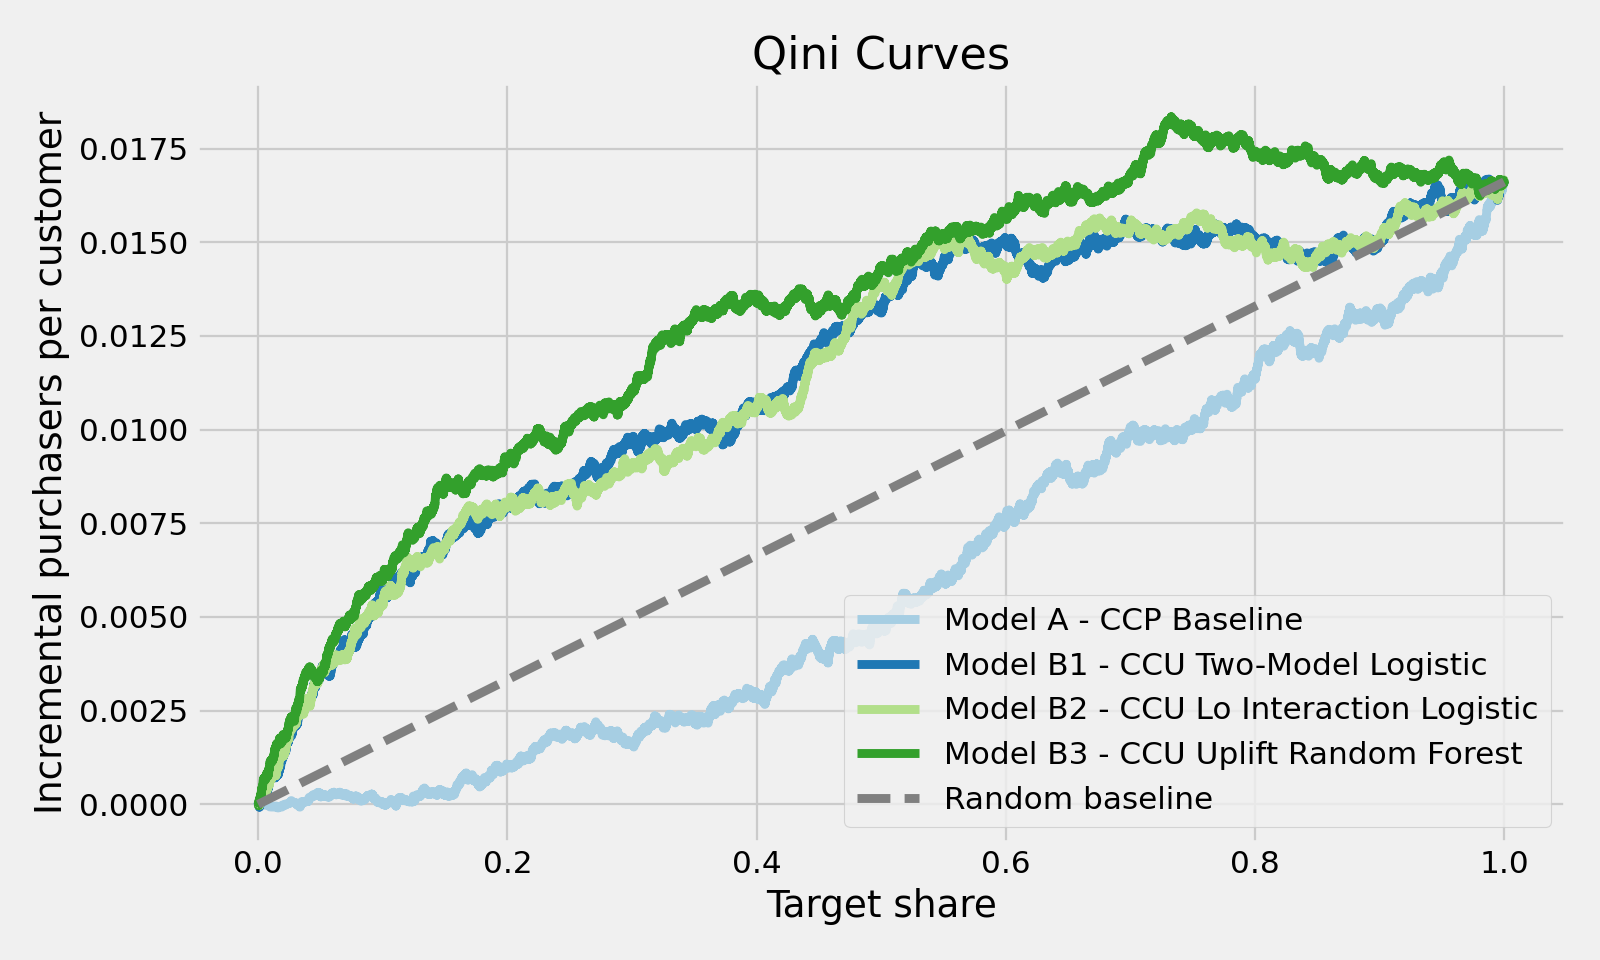
\includegraphics[width=0.88\textwidth]{report_assets/qini_curves.png}
\caption{Qini curves on the Phase II validation holdout.}
\label{fig:qini}
\end{figure}

Figure~\ref{fig:liftup} shows the liftup curves. The CCP baseline has very high top-decile response lift but almost no top-decile liftup, which is precisely the failure mode Phase I warned about.

\begin{figure}[H]
\centering
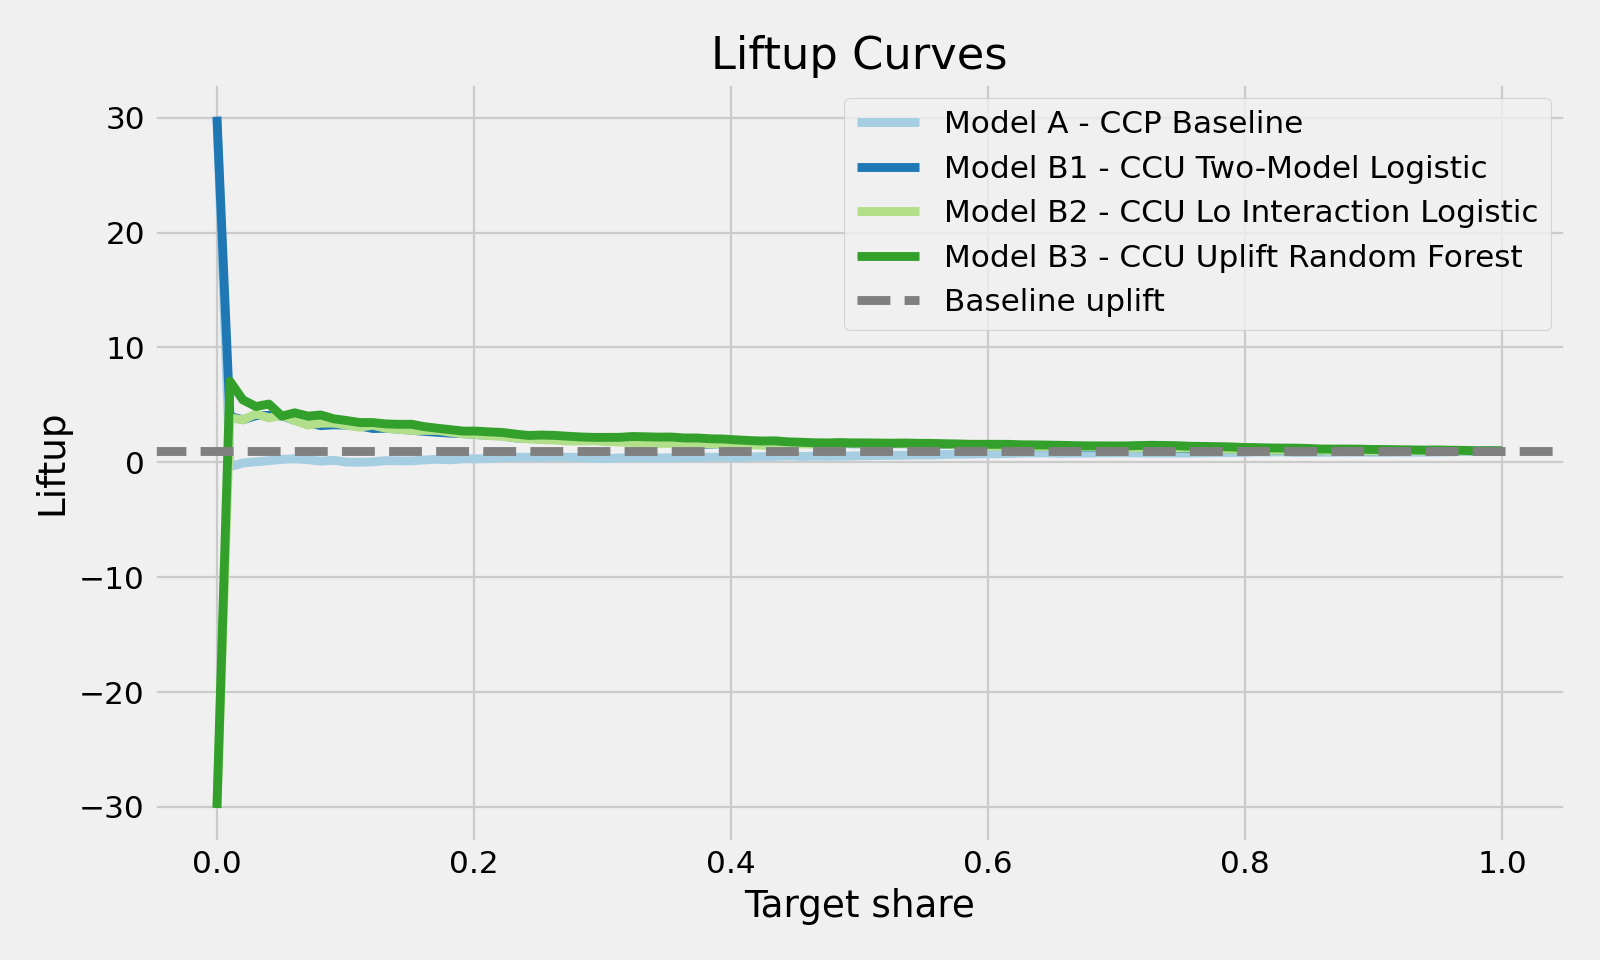
\includegraphics[width=0.88\textwidth]{report_assets/liftup_curves.png}
\caption{Liftup curves on the Phase II validation holdout.}
\label{fig:liftup}
\end{figure}

Figure~\ref{fig:profit} compares incremental profit curves and the CCP predictive MP curve. The uplift random forest is the only model that clearly pushes the incremental-profit frontier upward.

\begin{figure}[H]
\centering
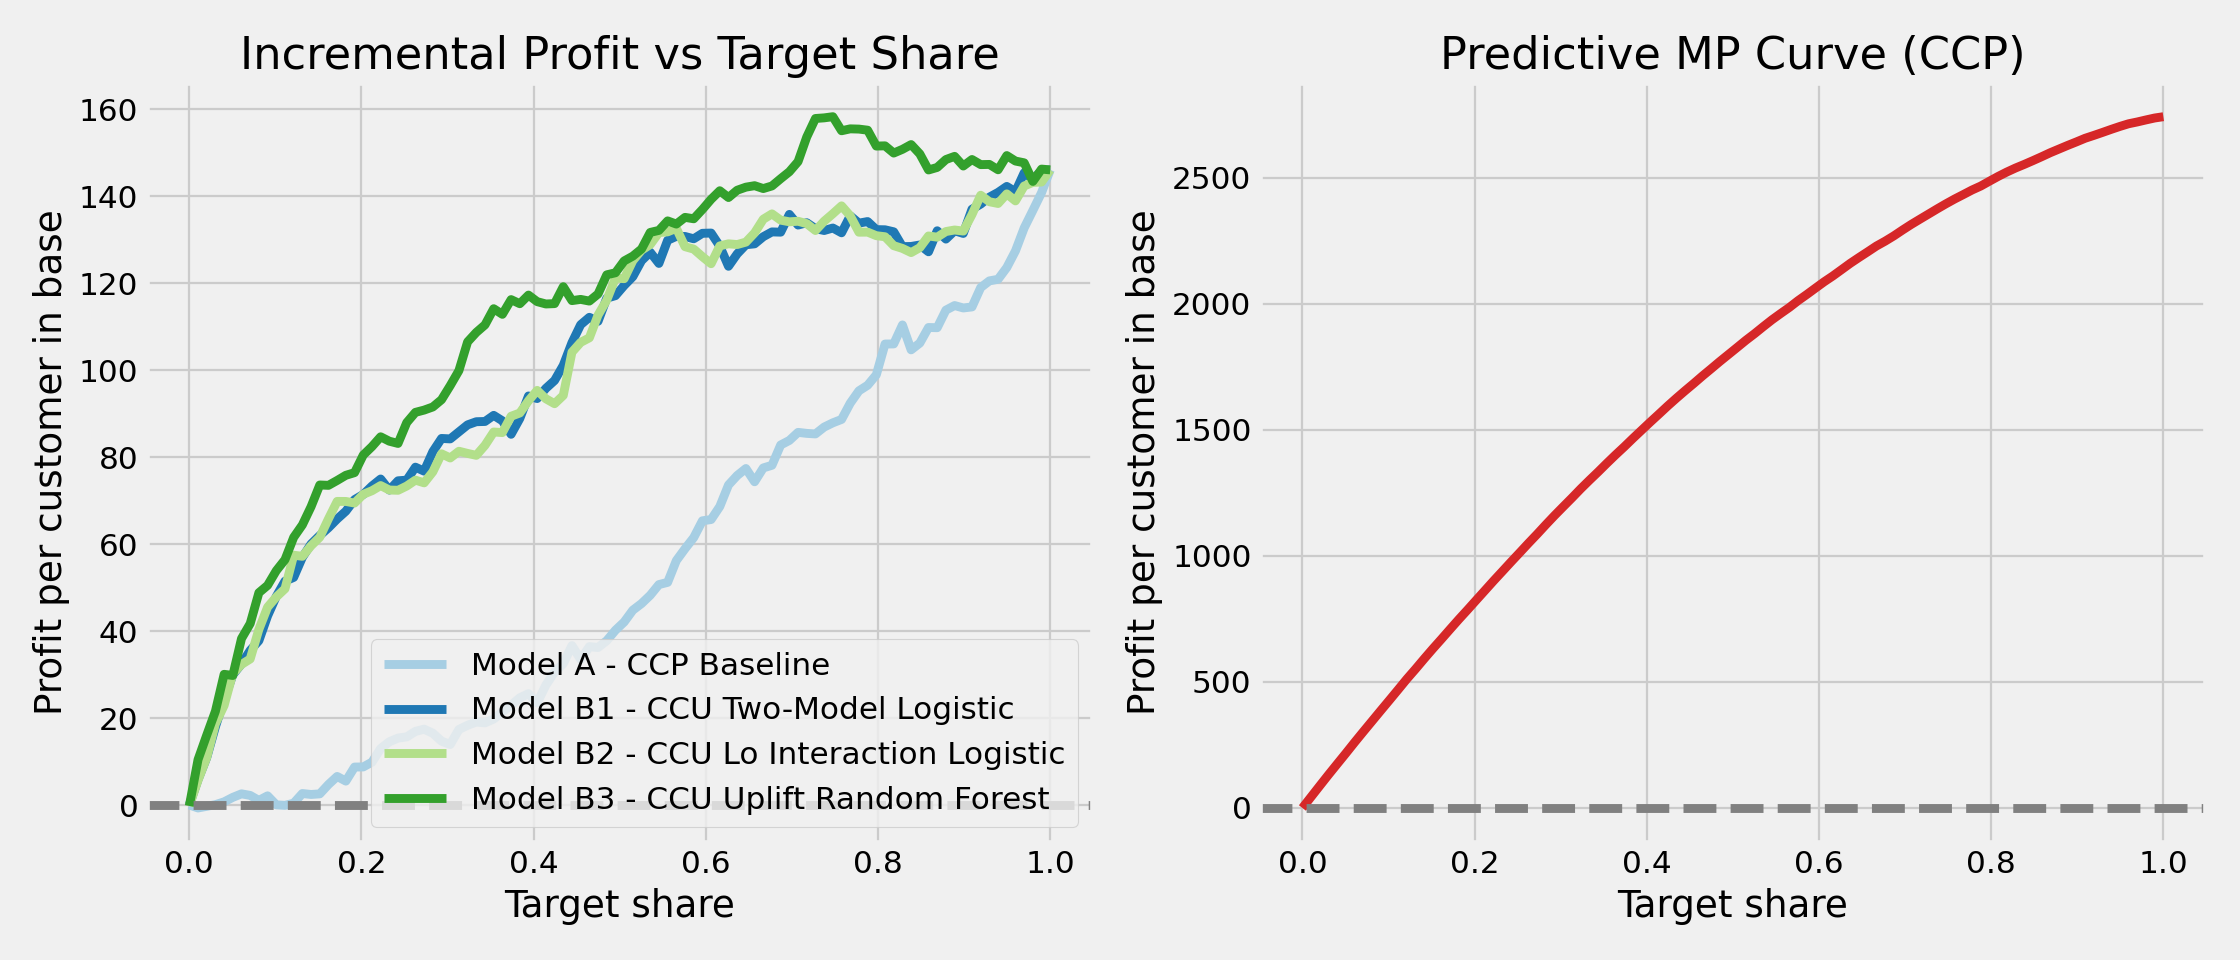
\includegraphics[width=0.92\textwidth]{report_assets/profit_vs_target_depth.png}
\caption{Incremental profit and CCP predictive MP curves.}
\label{fig:profit}
\end{figure}

Figure~\ref{fig:sensitivity} shows that the relative ordering is not a single-point artifact of the chosen economics; the uplift random forest remains competitive under the current sensitivity sweep.

\begin{figure}[H]
\centering
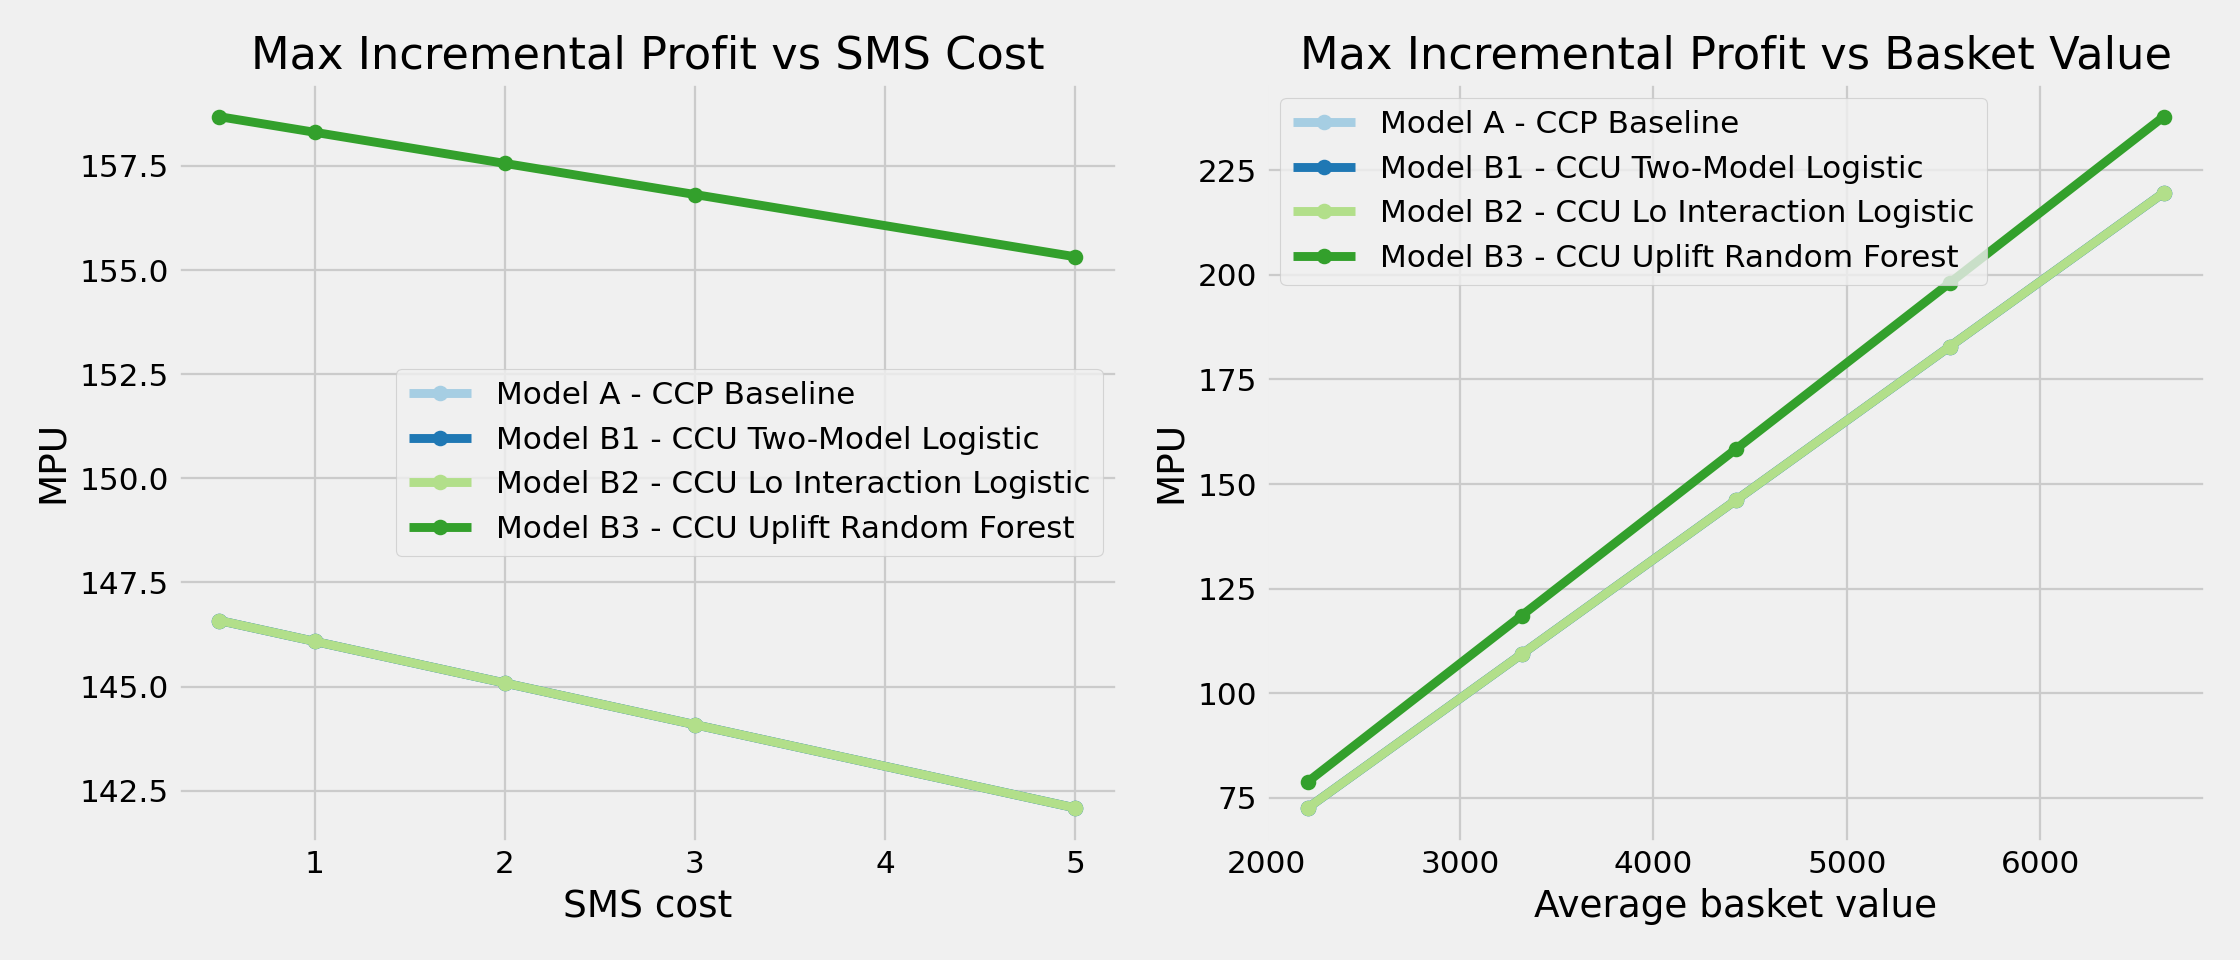
\includegraphics[width=0.92\textwidth]{report_assets/profit_sensitivity.png}
\caption{Sensitivity of maximum incremental profit to basket value and SMS cost assumptions.}
\label{fig:sensitivity}
\end{figure}

\section{Defense of the Work}
\subsection{Why the pipeline is methodologically sound}
The work is defensible because it avoids three common errors:
\begin{enumerate}
    \item \textbf{It does not confuse purchase likelihood with incremental value.}
    \item \textbf{It does not rely on notebook-only, hand-built outputs.}
    \item \textbf{It does not treat anonymized product categories as if they were interpretable business taxonomies.}
\end{enumerate}

Instead, the implementation follows the empirical evidence established in Phase I and uses a validation framework aligned with the targeting objective.

\subsection{Why the model comparison is fair}
The comparison is fair because:
\begin{itemize}
    \item all models use the same raw source data,
    \item all models use the same engineered feature base,
    \item all uplift models are tuned on inner splits only,
    \item all final metrics come from the same outer validation set.
\end{itemize}

\subsection{Why the conclusions are credible}
The conclusions are credible because they are supported simultaneously by:
\begin{itemize}
    \item Phase I causal balance checks,
    \item full-run validation outputs,
    \item uplift-specific ranking curves,
    \item profit-oriented summaries,
    \item formal verification scripts for both feature integrity and saved artifacts.
\end{itemize}

\section{Limitations}
The current work still has limits:
\begin{itemize}
    \item The hashed product hierarchy limits semantic interpretation.
    \item The current profit analysis depends on default economic assumptions, though sensitivity analysis reduces that risk.
    \item The uplift random forest uses a heavier third-party package and is slower than the logistic baselines.
    \item The implementation is an experimental analysis pipeline, not a production scoring service.
\end{itemize}

These limitations are acceptable at this stage because the objective of Phase II was comparative methodology and defensible empirical evidence, not deployment.

\section{Conclusion}
Phase II successfully translated the Phase I findings into a reproducible uplift-modeling comparison. The resulting pipeline demonstrates that:
\begin{itemize}
    \item a conventional CCP purchase-propensity ranking is not sufficient for incremental targeting,
    \item uplift-specific models are empirically justified on this dataset,
    \item the uplift random forest is currently the strongest model under the implemented evaluation framework.
\end{itemize}

The project therefore supports the central claim that targeting customers by expected incremental response is more defensible than targeting them by unconditional purchase probability alone.

\appendix
\section{Relevant Code Listings}
The report includes the most relevant implementation excerpts directly from the working codebase.

\subsection{Client and Product Feature Construction}
\lstinputlisting[
  style=pythonstyle,
  firstline=45,
  lastline=90,
  caption={Client-level feature construction in \texttt{phase2\_features.py}},
  label={lst:clientfeatures}
]{retailhero-uplift/phase2_features.py}

\lstinputlisting[
  style=pythonstyle,
  firstline=119,
  lastline=233,
  caption={Product-behavior aggregation and share-feature construction in \texttt{phase2\_features.py}},
  label={lst:productfeatures}
]{retailhero-uplift/phase2_features.py}

\subsection{Uplift Model Wrappers}
\lstinputlisting[
  style=pythonstyle,
  firstline=73,
  lastline=203,
  caption={Two-model logistic, interaction logistic, and uplift random forest wrappers in \texttt{phase2\_models.py}},
  label={lst:modelwrappers}
]{retailhero-uplift/phase2_models.py}

\subsection{Pipeline Orchestration}
\lstinputlisting[
  style=pythonstyle,
  firstline=167,
  lastline=340,
  caption={Main orchestration flow in \texttt{phase2\_pipeline.py}},
  label={lst:pipeline}
]{retailhero-uplift/phase2_pipeline.py}

\section{Reproduction Commands}
\begin{lstlisting}[style=pythonstyle,caption={Commands used to reproduce the work}]
cd "D:\Business Analytics\retailhero-uplift"
python -m pip install -r .\requirements.txt
python .\verify_phase1_findings.py
python .\phase2_pipeline.py --reuse-features
python .\verify_phase2_outputs.py
\end{lstlisting}

\begin{thebibliography}{9}
\bibitem{devriendt2021}
Devriendt, F., Guns, T., and Verbeke, W. (2021).
\newblock Learning to rank for uplift modeling.
\newblock In the value-driven uplift modeling literature adapted here for campaign targeting.

\bibitem{lo2002}
Lo, V. S. Y. (2002).
\newblock The True Lift Model.
\newblock A treatment-interaction approach to uplift-style modeling.
\end{thebibliography}

\end{document}
